\documentclass[pdftex,12pt,letter]{article}
\usepackage[binary-units=true]{siunitx}
\usepackage[margin=0.75in]{geometry}
\usepackage{verbatim}
\usepackage{graphicx}
\usepackage{cite}
\usepackage{color}
\usepackage[pdftex,pdfpagelabels,bookmarks,hyperindex,hyperfigures]{hyperref}
\usepackage{xspace}
\usepackage{amssymb}

\usepackage[firstpage]{draftwatermark}


\bibliographystyle{unsrt}

\newcommand{\fixme}[1]{\textbf{FIXME: #1}}    
\newcommand{\pd}{protoDUNE\xspace}

\title{A proposal for the Single-Phase \pd (NP04) data challenges in 2017-2018}
\date{\today}
\author{R.Pordes, M.Potekhin, D. Stefan, R.Sulej}

\begin{document}
\SetWatermarkText{DRAFT}
\SetWatermarkLightness{0.9}
\SetWatermarkScale{3}

\maketitle

\begin{abstract}
\noindent There are two main factors that compell the \pd collaborators to take necessary mesaures
to ensure 100\% readiness of the whole \pd software and computing complex during most of the
commissioning period and throughout data taking in 2018. First, due to the short run schedule the beam
time is precious and spending any significant amout of time on debugging will make fulfillment of
the run plan impossible. Second, the Collaboration will need to process and analyze the NP04 data
on a reasonably short time scale (months rather than years) in order to maximize benefits of the
prototype effort for the DUNE R\&D work and CDR cycle, so efficient resource management and
throughput of \pd processing will be of essence right at the beginning of data taking. For these
reasons, and given the \pd schedule,  we propose to conduct two Data Challenges in order to identify
and address potential issues before they can impact the experiment.



\end{abstract}

\tableofcontents

\pagebreak

\section{About this document}
%The Single-Phase \pd experiment (NP04) is characterized by substantial data rates
%and volume, as well as by inherent complexity of its data handlng and processing scheme due
%to properties of its main detector (the Liquid Argon TPC), readout electronics and other factors.
%Initial estimates indicate considerable CPU and storage requirements for production and analysis.
%In order to ensure readiness of the protoDUNE computing infrastructure for data taking
%in 2018, it will be necessary to conduct Data Challenges which are meant to validate
%individual infrastructure and software components, interfaces  as well as the status of overall
%system integration.
The goal of this document is to provide concise information about the proposed \pd Data Challenges
to the infividual working groups in order to coordinate effort and come to a consensus as to the scope,
plans and schedule of the proposed Data Challenges. It does not contain detailed descriptions
and/or designs of the \pd computing
infrastructure elements and the reader is reffered to existing documentation where
needed, with references provided in the text.

\section{The Scope of the Data Challanges}
Information regarding the \pd (NP04) computing is summarized in the \pd-SP Technical Design Report\cite{docdb1794}.
The following components can be identified as relevant in the context of Data Challanges:
\begin{itemize}
\item The DAQ \textbf{Online Buffer} which stores raw data assembled by the Event Builders, as files on disk. The internals
of the DAQ system itself are not within the scope.

\item The \textbf{Raw Data Handling System}\cite{docdb1212}  which performs data transfers between a few endpoints
at CERN and FNAL starting with the Online Buffer and which is also tasked with proper accounting and handling of Metadata
by interacting with the SAM system at FNAL (see next item). The Data Handling System will inteface the disk-based mass storage
at CERN and FNAL (i.e.\,EOS and dCache) as well as tape systems (CASTOR and Enstore). We anticipate using the \textit{Fermi
File Transfer System}\cite{fts} for most of this functionality.

\item The \textbf{Metadata}  -- SAM system at FNAL which comprises the functionality of the file catalog, data storage and
retrieval based on Metadata and can also be used for orchestration of production workflows.

\item \textbf{Data Quality Monitoring} (DQM) which is tasked with running algorithms with turnaround time short enough to provide
actionable results (under and hour) but which won't fit into the computational footprint of the Online Monitoring (a part of DAQ).
To support DQM, the ProtoDUNE Prompt Processing System (\textbf{p3s}) has been created and will run any type of DQM workload
as requested by the working groups.

\item \textbf{Calibration and Production}. While it is not expected that these components will be finalized for at least the first Data
Challenge it is important to have a firm grasp of the required interfaces, data flow patterns and other crucial aspects of
the \pd Production Systems. Having functional prototypes in place is therefore crucial on the time scale of the Data Challenges.
An important component of the overall production chain is the \textit{Data Reduction} step along the lines described
in \cite{docdb2089}. In one shape or another it is likely to be included in the production software and will in fact constitute
one of the more CPU-intensive components. Understanding the interfaces and practical implications of this component would
be a useful part of the Data Challenge.

\item \textbf{Analysis Suite Prototypes}. Same comment applies here as to the previous item, i.e.\, while there is no expectation
for the final design and implementation of the analysis chain to exist (especially that it's by nature the most dynamic part of all
software) it is important to put in place, document and optimize its interfaces with various components of infrastructure e.g.\,calibration
databases, Metadata, software and data provenance controls etc.

\end{itemize}
\noindent Relationship between the infrastructure and other components listed above is schematically illustrated in
Fig.\ref{fig:dc1}.

\begin{figure}[tbh]
  \centering
  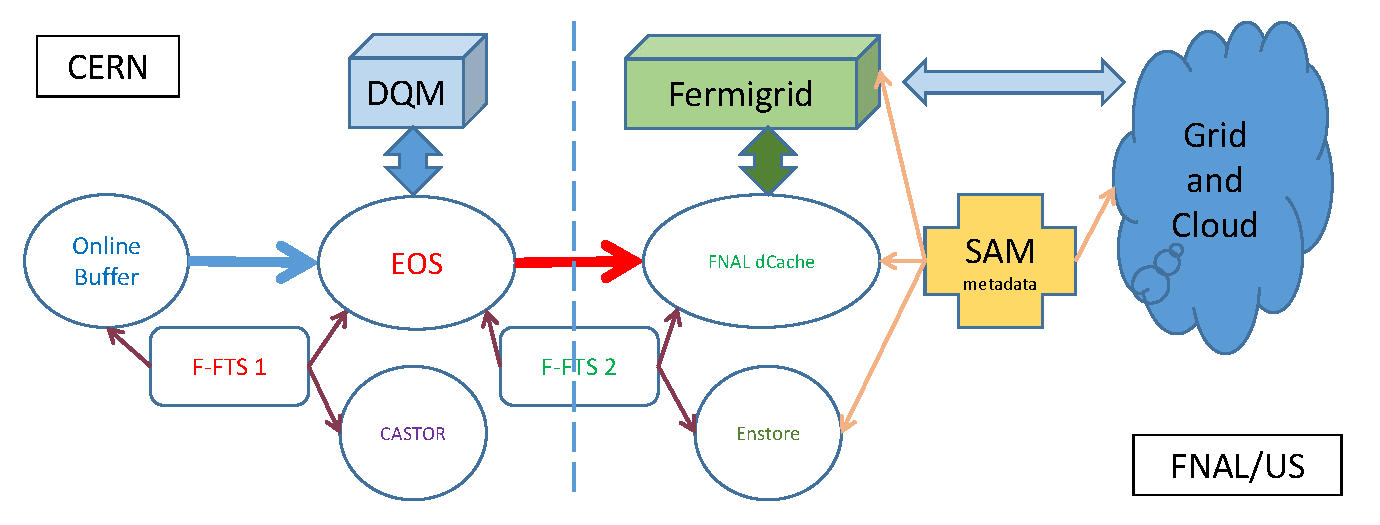
\includegraphics[width=1.0\textwidth]{figures/data_challenge_1.pdf}
  \caption{Schematics of data flow and  processing in \pd data challenges.}
  \label{fig:dc1}
\end{figure}

\section{Timeline and Milestones}
\label{sec:timeline}
The items below include system deployment, functional and integration testing.
Critical milestones are marked by bullets.

\begin{description}

\item[Feb'17: initial prototype] --- a working instance of p3s having most of
required functionality, utilizing the ``Django development server'' and \textit{sqlite}
database back-end.

\item[Mar'17: Apache/PostgreSQL] --- a continuously running instance of
p3s deployed on Apache with PostgreSQL back-end, in a test setup at BNL.
Resolution of concurrency issues.

\item[Apr'17: initial CERN deployment] --- p3s deployed on the DQM (\textit{neutdqm}) cluster.

\item[May'17: XRootD] --- XRootD service on the DQM cluster with
a functioning interface to EOS.

\item[Jun'17: payload integration] --- art/LArSoft payloads confugured to run on p3s; system
 automated data driven generation and management of workflows
\begin{itemize}
\item DAQ vertical slice readiness
\end{itemize}

\item[Jul'17: Visual and Data Products] --- Web server optimized
for delivery of visual and data products produced by p3s.


\item[Sep'17: p3s/DAQ integration testing] --- 
\begin{itemize}
\item Full DAQ test readiness
\end{itemize}

\item[Q4'17] --- p3s stress and scalability testing, additional development

\item[Q1'18] --- continuous p3s operation with realistic workloads, running
MC/Reco jobs in utility mode

\item[Q2'18]\ 
\begin{itemize}
\item Full data taking readiness
\end{itemize}

\end{description}


\section{Resources}
\label{sec:resources}

\subsection{Effort Levels}

Development/engineering
\begin{itemize}
\item M.Potekhin (BNL), lead developer --- 100\%\,FTE
\item B.Viren (BNL), design consultant --- 10\%\,FTE
\end{itemize}

\noindent System administration and support (working assumption)

\begin{itemize}
\item M.Potekhin (BNL) --- deployment and general maintenance
\item Modest contributions to the p3s support and maintenance are tentatively anticipated from N.Benekos (CERN) and G.Savage (FNAL)
however the actual effort level is subject to discussion with all parties involved.
\end{itemize}

\noindent The amount of effort needed for development of payload jobs
is not considered in scope but see above sections for a discussion of
how the DQM group will contribute and assist.

\subsection{Mat\'eriel}

A rough guess is that at a minimum the DQM payload jobs running on p3s will require O(100)
cores during its operation.  This is an elastic requirement.  More available
cores will allow more intensive processing over a larger percentage of
the raw data while restricting the available hardware can be met by a
scaling back.  This scaling is automatically achieved by p3s. Separately,
a small number of adequately speced and configured machines are needed for
deployment of Web and DB servers to support the p3s function.  

It is a working assumption at the time of writing that a significant
portion of the \textit{neut} cluster \cite{neut} will be assigned for
p3s use as \pd ramps up its operations in 2017 and into 2018.  However
and in any case the DQM group relies on \pd management to assist in
finding suitable computing resources, especially in securing a guaranteed
resource allocation on \textit{lxbatch} if the Beam Instrumentation
processing is to run on that facility.


\section{Risk Assessment}
\label{sec:risk}

Technologies used in p3s are not new, they are mature and tested in the field, which reduces
overall implementation risk. The remaining risk factors are
\begin{itemize}

\item Integration of the Beam Instrumentation Data. The amount
of development work necessary to access these data is not well
understood. Optimal design of the merging process (e.g. to avoid
doubling the data volume while writing out the merged data)
can be a challenge.

\item Insufficient allocation of hardware to p3s jobs can reduce
  the amount of data processed or the capability of the allowed
  algorithms to such an extent that the fraction of triggers or the
  types of features in the data which can be checked leads to a
  failure to identify problems in the detector.

\item Lack of coordination and identification of individuals to
  develop the payload jobs which have sufficient coverage and
  performance may likewise lead to failure to identify problems in the
  detector.


\item DQM relies on the DAQ group to release updates to the ``data
  access library'' needed for unpacking raw data in a manner prompt
  enough so that p3s payload jobs can adapt, be rebuilt and deployed.
  Failures in this chain can lead to periods of time where detector
  data is unreadable and no data quality monitoring results are
  produced.

\item If the small subsamples of the initial raw data is ingested from
  EOS then DQM results depend on the successful and prompt transfer of
  raw data files from the Online Buffer to EOS by F-FTS.  Any delay or
  outage will translate to late or missing DQM results.

\item If initial and ongoing sysadmin support is
  not allocated for the p3s worker nodes and the
  p3s web and database servers then the system deployment
  may be delayed and/or unreliable.

\end{itemize}

\clearpage
\begin{thebibliography}{1}

\bibitem{docdb1794}
{DUNE DocDB 1794: \textit{ProtoDUNE-SP Technical Design Report }}\\
\url{http://docs.dunescience.org:8080/cgi-bin/ShowDocument?docid=1794}



\bibitem{docdb1212}
{DUNE DocDB 1212: \textit{Design of the Data Management System for the protoDUNE Experiment}}\\
\url{http://docs.dunescience.org:8080/cgi-bin/ShowDocument?docid=1212}

\bibitem{fts}
{The Fermilab File Transfer System}\\
\url{http://cd-docdb.fnal.gov/cgi-bin/RetrieveFile?docid=5412&filename=datamanagement-changeprocedures.pdf&version=1}



\bibitem{docdb2089}
{Proposed Initial Data Reduction for protoDUNE/SP}\\
\url{http://cd-docdb.fnal.gov/cgi-bin/RetrieveFile?docid=2089&filename=datamanagement-changeprocedures.pdf&version=1}


\bibitem{xrootd}
{XRootD}\\
\url{http://www.xrootd.org}

\bibitem{eos}
{The CERN Exabyte Scale Storage}\\
\url{http://information-technology.web.cern.ch/services/eos-service}



\bibitem{docdb1811}
{DUNE DocDB 1811: \textit{Prompt Processing System Requirements for the Single-Phase protoDUNE}}\\
\url{http://docs.dunescience.org:8080/cgi-bin/ShowDocument?docid=1811}



\bibitem{neut}
{Neutrino Computing Cluster at CERN}\\
\url{https://twiki.cern.ch/twiki/bin/view/CENF/NeutrinoClusterCERN}

\bibitem{lxbatch}
{The CERN batch computing service}\\
\url{http://information-technology.web.cern.ch/services/batch}

\bibitem{django}
{Django}\\
\url{https://docs.djangoproject.com/en/1.10/}


\bibitem{docdb1086}
{DUNE DocDB 1086: \textit{ protoDUNE/SP data scenarios with full stream (spreadsheet)}}\\
\url{http://docs.dunescience.org:8080/cgi-bin/ShowDocument?docid=1086}




\end{thebibliography}


\end{document}

%%% Local Variables:
%%% mode: latex
%%% TeX-master: t
%%% End:
\grid
